\documentclass{standalone}

\usepackage{pgfplots}
\pgfplotsset{compat=newest}
\usepackage{tikz}
\usetikzlibrary{decorations.markings}
\usetikzlibrary{patterns}
\usetikzlibrary{fillbetween}


\begin{document}



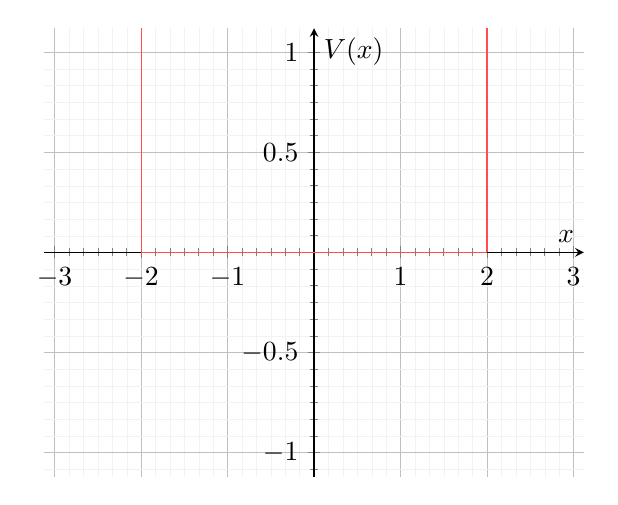
\begin{tikzpicture}

\tikzset{
	hatch distance/.store in=\hatchdistance
	hatch distance=10pt
	hatch thickness/.store in=\hatchdistance
	hatch thickness=2pt
}

  \begin{axis}%
    [grid=both,
     minor tick num=5,
     xlabel=$x$,
     ylabel=$V(x)$,
     grid style={line width=.1pt, draw=gray!10},
     major grid style={line width=.2pt,draw=gray!50},
     axis lines=middle,
     restrict y to domain=0:15.,
     enlargelimits={abs=1.12}
    ]
    \addplot[domain=-2:2,samples=50,smooth,red!70] {0} ;
    \draw[red!70] (2, -0.) -- (2, 10);
    \draw[red!70] (-2, -0.) -- (-2, 10);
    %\addplot+[mark=none, 
	    %domain=-1:1,
	    %samples=50,
	    %hatch distance=5pt,
	    %hatch thickness=0.5pt,
	    %draw=red!70,
	    %pattern color=blue,
	    %area legend] {(1-cos(deg(pi*x)))/(1+cos(deg(pi*x)))} \closedcylcle;
  \end{axis}
\end{tikzpicture}



\end{document}

